\section{Conventions}

\np To differentiate the concepts and terminologies in the Dats language and
actual music terms, we prefix "musical" to any terms and concepts which
refers to the actual concepts in music. For example, \textit{musical staff} refers
to the five line-staff in western musical notation, while \textit{staff} refers to
the concept of staff keyword describe in this document. Similarly,
\textit{musical note} and \textit{musical rest} refers to the symbol of a musical
sound and symbol of silence in the field of music\footnote{\textit{Musical note} and
\textit{musical rest} might also be use interchangeably with the statements in a
\textit{staff block}.} while \textit{note} in this Dats language refers to the literal
consisting of a key, an optional accidental, and an octave, \protect\texttb{[a-g](b|\#)?[0-9]}.
 
\np Figures of musical staffs presented throughout this document follows the
western musical notation of five line-staff. In a G-clef, each respective
spaces are note of f4 a4 c5 e5:

\begin{center}
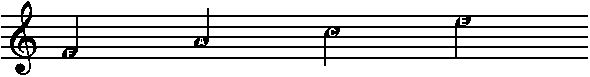
\includegraphics{notes/face}
\end{center}

and the lines are of e4 g4 b4 d5 f5:

\begin{center}
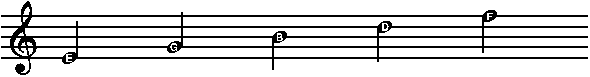
\includegraphics{notes/egbdf}
\end{center}

Any figure which reference to this five line staff refers to the convention above.

\np 
Numbered paragraphs introduces concepts independent of the previous paragraphs.
Examples provide possible forms of the constructs described. Words in \textgray{grey boxes}
are interpreted as keyword of the language. \texttb{Bolded teletype} words signifies piece of code 
formatted for emphasis.  \textit{Italicized} words groups technical words together as one
concept and also serve as emphasis. Words enclosed in a less-than sign and greater-than sign are
interpreted as \texttb{<arguments>}.

Section 4 gives the readers an overview of the language. Section 5 and the next proceeding sections
gives formal definition of the language, its syntax and semantics.



